\documentclass{article}
\usepackage[T1]{fontenc}
\usepackage[utf8]{inputenc}
\usepackage[a4paper, total={6in, 8in}]{geometry}
%\usepackage[icelandic]{babel}
\usepackage{graphicx} %package to manage images

\usepackage{hyperref}
\usepackage{siunitx}
\usepackage{tabularx}

\usepackage{xcolor}
\usepackage{listings}

\colorlet{mygray}{black!30}
\colorlet{mygreen}{green!60!blue}
\colorlet{mymauve}{red!60!blue}

\lstset{
  backgroundcolor=\color{gray!10},  
  basicstyle=\ttfamily,
  columns=fullflexible,
  breakatwhitespace=false,      
  breaklines=true,                
  captionpos=b,                    
  commentstyle=\color{mygreen}, 
  extendedchars=true,              
  frame=single,                   
  keepspaces=true,             
  keywordstyle=\color{blue},      
  language=c++,                 
  numbers=none,                
  numbersep=5pt,                   
  numberstyle=\tiny\color{blue}, 
  rulecolor=\color{mygray},        
  showspaces=false,               
  showtabs=false,                 
  stepnumber=5,                  
  stringstyle=\color{mymauve},    
  tabsize=3,                                     
  title=\lstname 
}

\title{Embedded Group Project\\ \large Project 4 - Kernel Space Encoder}

\author{Steinarr Hrafn Höskuldsson\\
Arnþór Gíslason\\
Andrew Madden\\
\\
Reykjavik University}
\date{October 2022}


\newcommand{\mycomment}[1]{}
\newcommand{\timerinterval}{5ms }

\begin{document}
\maketitle
 % how to comment, input image and code
\mycomment{
\begin{figure}[h]
    \centering
    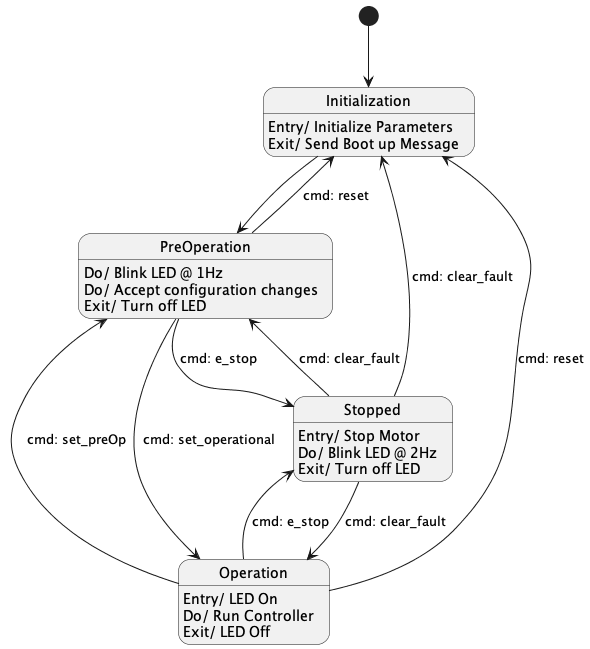
\includegraphics[width=0.75\textwidth]{Project3ControllerStateMachine/out/Project3ControllerStateMachine/docs/uml/uml.png}
    \caption{UML}
    \label{fig:UML}
\end{figure}

\lstinputlisting[caption=Defining 'ColorMatch' state, label={lst:colormatch}, language=Python, firstline=44, lastline=52]{LAB3/Basic.py}

}

\section{Part 1}
The header pins were soldered onto the Raspberry Pi Zero W2 and a voltmeter used to check that the pin orientation was correct.
\section{Part 2}
The four different methods for interfacing with the GPIO pins were tested.
\subsection{Test Setup}
A function generator ( WHAT MODEL?) was hooked up to pin ????????? and set to output a square wave with amplitude 3 volts and frequency 1kHz. A Rhode\&Schwartz RBT2004 oscilloscope was used to probe the input and output pins on different channels. The oscilloscope was then set to measure the time difference between rising edges.

With each method a screenshot of the oscilloscope was taken and the CPU load was read by running top in another terminal window.

\subsection{Using sysfs from a shell script}

\begin{figure}[h]
    \centering
    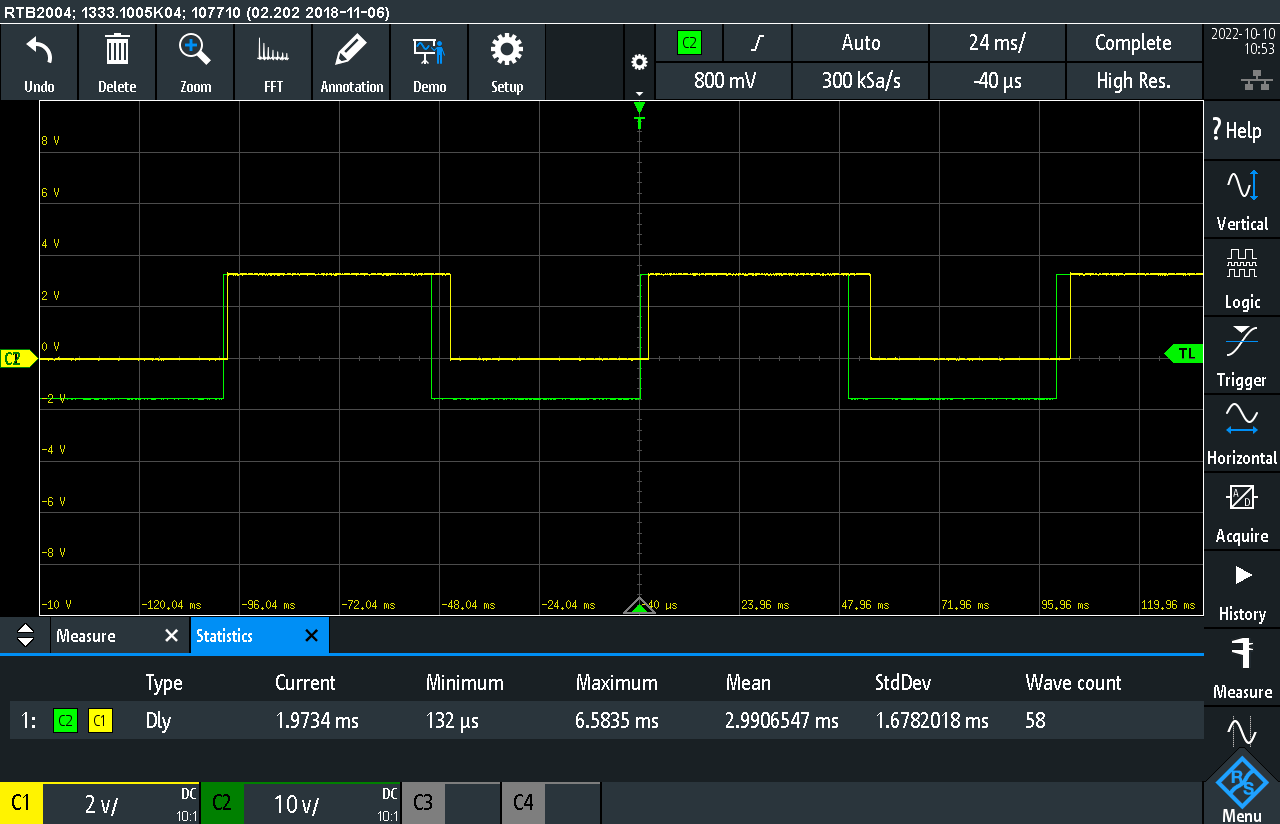
\includegraphics[width=0.75\textwidth]{Project4KernelSpaceEncoderDriver/part2_shell_mirror.PNG}
    \caption{Response time of a shell script utilizing sysfs to mirror a pin}
    \label{fig:shell}
\end{figure}
The CPU usage of the bash script was around 19\%.

\subsection{Using sysfs from a C/C++ application}

The CPU usage of the program was 100\%

\subsection{Using sysfs and poll() from a C/C++ application}

The CPU usage was 0.3\%

\subsection{A kernel module using interrupts}





\subsection{Discussion}
The minimum response time needed is ?????? microseconds (MAYBE QUOTE PREVIOUS REPORT?) therefore something something

\section{Part 3}

\begin{figure}[h!]
    \centering
    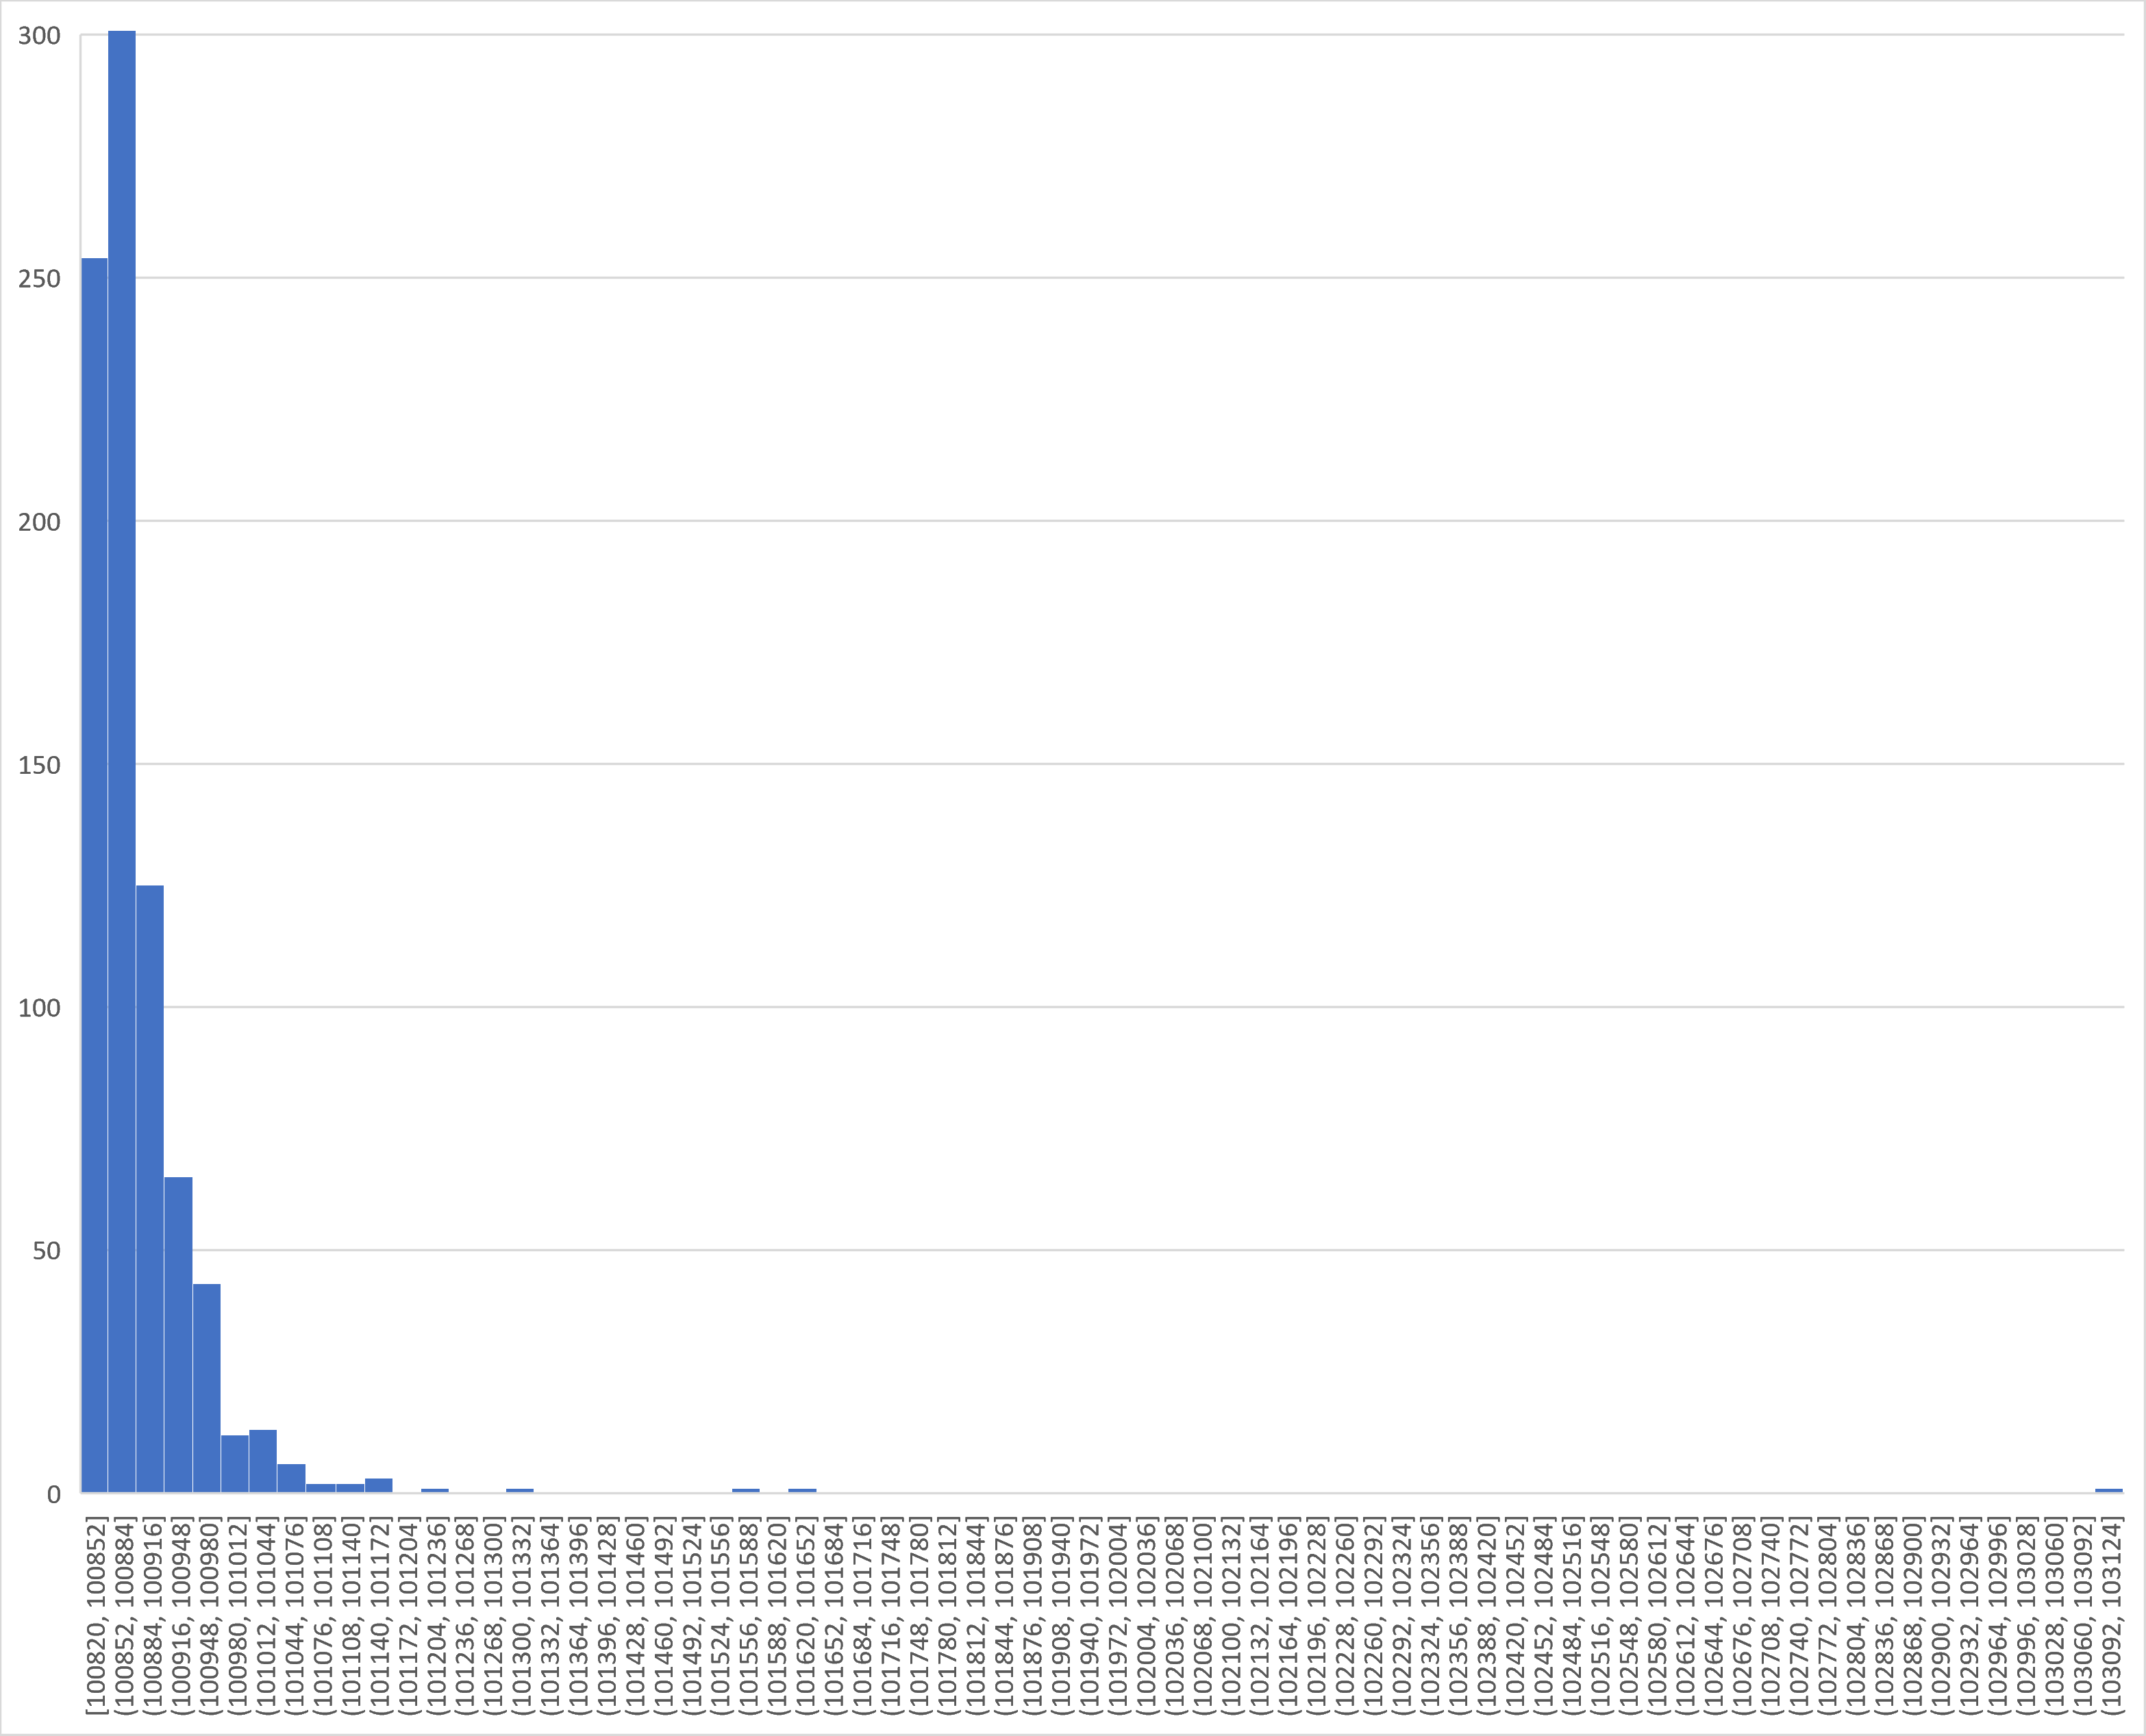
\includegraphics[width=0.75\textwidth]{Project4KernelSpaceEncoderDriver/histogram_timebetweenruns.png}
    \caption{histogram plot of delta time between runs of the PI controller}
    \label{fig:histogramDelta}
\end{figure}
\begin{figure}[h!]
    \centering
    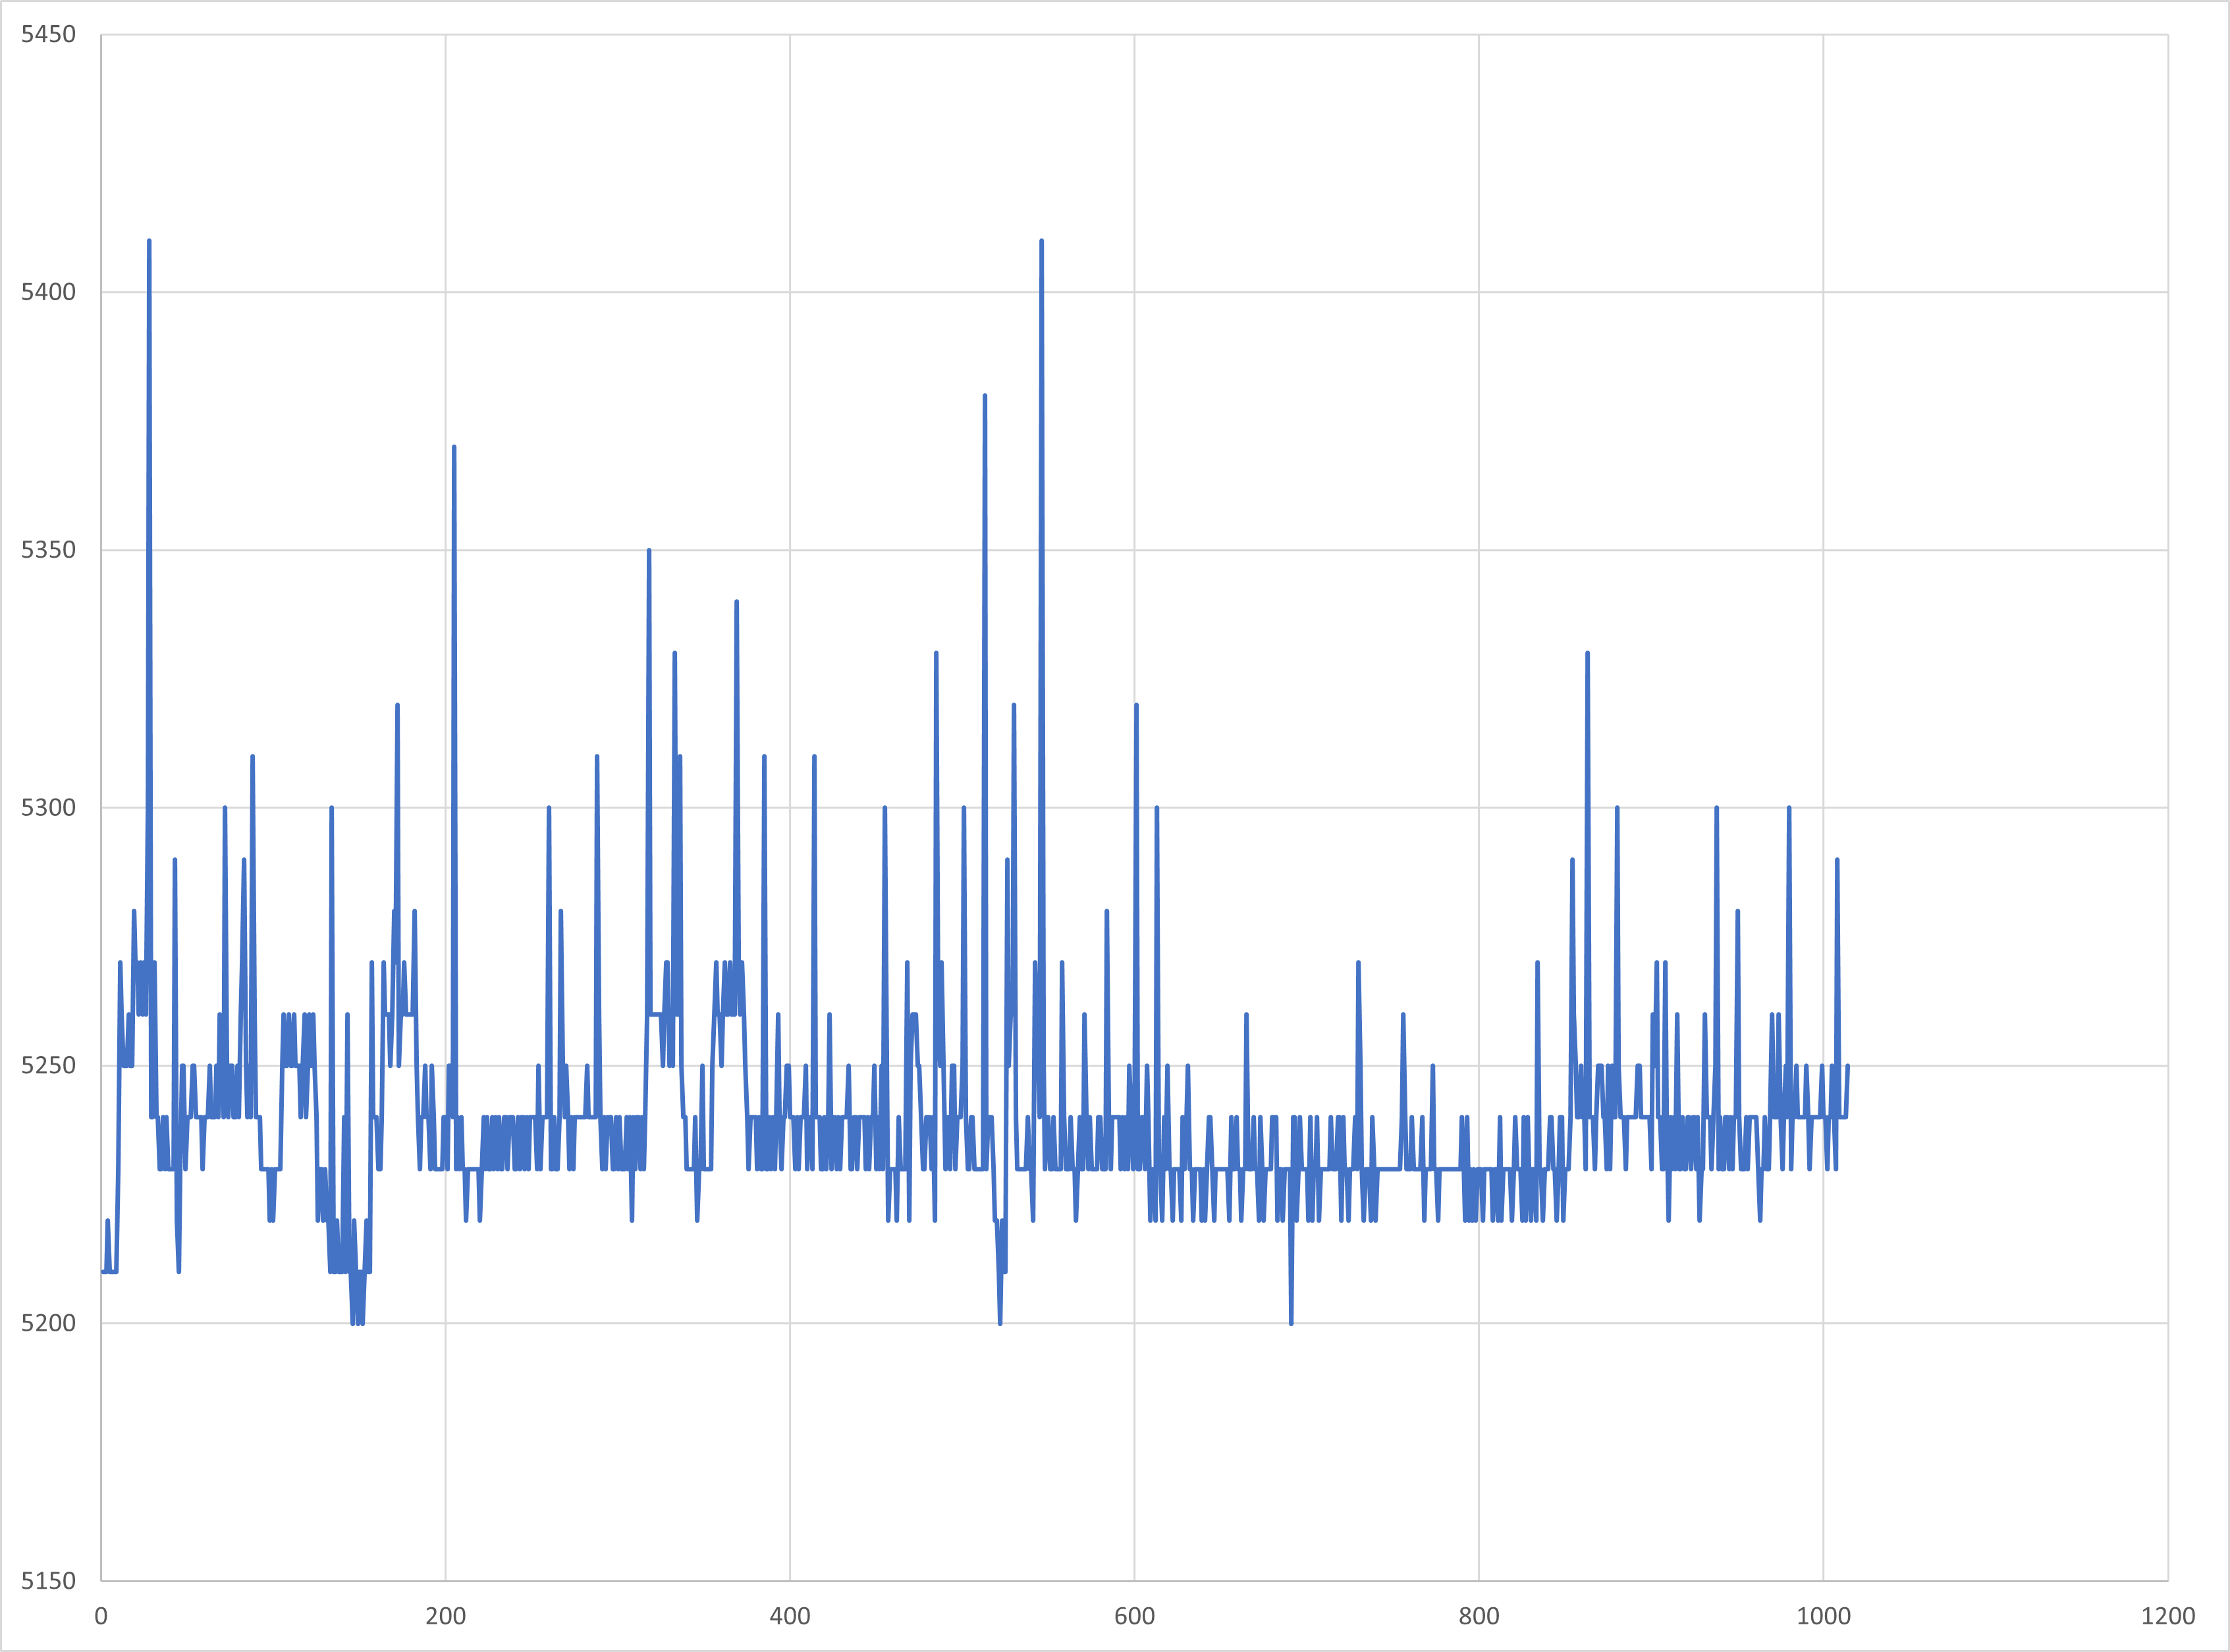
\includegraphics[width=0.75\textwidth]{Project4KernelSpaceEncoderDriver/scatterplot_between_runs.png}
    \caption{histogram plot of delta time between runs of the PI controller}
    \label{fig:scatterplotDelta}
\end{figure}
\newpage
\section*{Appendix}
\appendix

\newpage
\section{Code}\label{appendix:code}

\lstinputlisting[caption=main program used to produce the step response]{Project2SpeedController/src/main.cpp}

\lstinputlisting[caption=timer\_msec.cpp]{Project1RotaryEncoder/src/encoder_simple.cpp}

\lstinputlisting[caption=main.cpp]{Project1RotaryEncoder/src/main.cpp}

\end{document}
